\documentclass[compress]{thesisbeamer}
\useoutertheme[subsection=false]{miniframes}
\usepackage{nccmath}
\usepackage{mathtools}
\usepackage[thinc]{esdiff}

\title{A Gazebo Simulator for Continuum Parallel Robots}
\author[Gotelli Andrea]{Author Gotelli Andrea\newline ~ \newline \normalsize{Advisors: Duh, Dih, Dah}}
\date{22/02/2021}

\bibliography{../biblio}

% video will work on Linux (with Okular) or OS X, for other OS's or viewers find your own way to do it
%\videoOSX	% for OS X 
%\videoOFF
\begin{document}

\MakeTitleNoFoot

    
   	\section{Introduction}
        \subsection{Serial_parallel_robots}
        \frametitle{Serial and parallel robots}
        \begin{frame}
            \begin{columns}
			\column{0.5\textwidth}
			\begin{itemize}%[<+->]
  				\item Serial robots
  				\begin{itemize}%[<.->]
   					\item Simpler and more used
   					\item Limited by precision and inertia
  				\end{itemize}\vfill
  				\item Parallel robots
  				\begin{itemize}%[<.->]
   					\item Less inertia, high velocities
   					\item More joints involved
  				\end{itemize}\vfill
 			\end{itemize}
			\vspace{2cm}
			\column{0.5\textwidth}
			\begin{figure}[h]
				\centering
				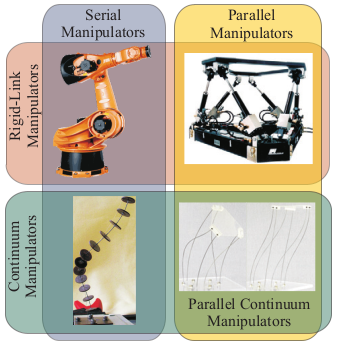
\includegraphics[width=\textwidth]{images/serial_parall_robots}
				\caption{Different robot architectures}
			\end{figure}
			\end{columns}
		\end{frame}

        \subsection{CPR}
        \begin{frame}
        	\frametitle{Continuum parallel robots}
			\begin{columns}
			\column{0.5\textwidth}
			\begin{itemize}%[<+->]
  				\item Continuum parallel robots 
  				\begin{itemize}%[<.->]
   					\item May anhance safety
   					\item Cheaper components 
   					\item Possible to miniturize
  				\end{itemize}
  				\item Model and stability problems
  				\begin{itemize}%[<.->]
   					\item More unstable configurations
   					\item Another drawback
   					\item Not analytical solution
  				\end{itemize}
 			\end{itemize}
			\vspace{2cm}
			\column{0.5\textwidth}
			\begin{figure}[h]
				\centering
				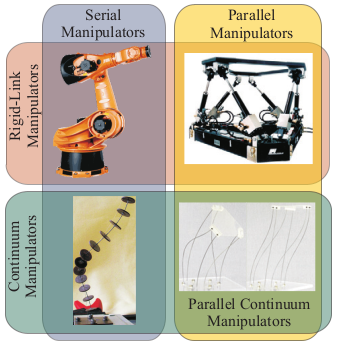
\includegraphics[width=\textwidth]{images/serial_parall_robots}
				\caption{Different robot architectures.}
			\end{figure}
			\end{columns}
		\end{frame}
		
		\subsection{CPR_simulator}
        \begin{frame}
        	\frametitle{CPR simulator}
			\begin{itemize}%[<+->]
  				\item General simulator 
  				\begin{itemize}%[<.->]
   					\item Gazebo
   					\item Different robots
  				\end{itemize}
  				\item Solve the modelling
  				\begin{itemize}%[<.->]
   					\item Rod statics
   					\item Robot assembly
   					\item Visual interface
   					\item Robot dynamics
  				\end{itemize}
  				\item Modelling of continuum
 			\end{itemize}
		\end{frame}


        \section{Methods}
        	\subsection{Geometric_modelling}
        	\begin{frame}
        		\frametitle{Geometric modelling}
				\begin{columns}
				\column{0.5\textwidth}
				\begin{itemize}%[<+->]
  					\item Rod as 1D body 
  					\item Function of the arc-lenght $ s $
  					\begin{itemize}%[<.->]
   						\item Centerline position $ p_{(s)}\in\mathbb{R}^3$
   						\item Cross-section orientation $ R_{(s)}\in\textit{se}(3)  $
  					\end{itemize}
  					\item Define transformation
  					\begin{equation}
  						T_{(s)} = 
  						\begin{bmatrix}
  							R_{(s)} & p_{(s)} 	\\
  								0	&	1		\\
  						\end{bmatrix}\in SE(3)
  					\end{equation}
  					\item Derivative wrt arc-lenght $ x^{'} = \diff{x}{s} $
 				\end{itemize}
				\vspace{2cm}
				\column{0.5\textwidth}
				\begin{figure}[h]
					\centering
					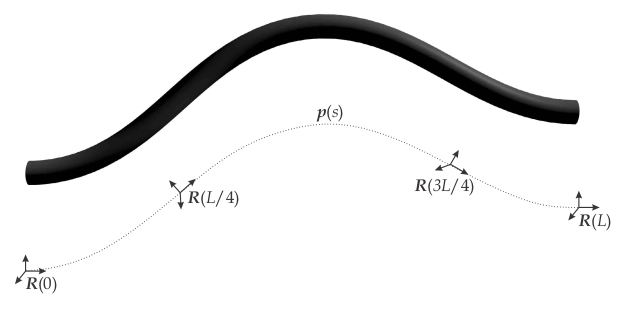
\includegraphics[width=\textwidth]{images/rod_geometry}
					\caption{Rod geometric modelling}
				\end{figure}
				\end{columns}
			\end{frame}

        \subsection{Rod_equilibrium}
        \begin{frame}
        	\frametitle{Equilibrium Equations}
			\begin{columns}
			\column{0.5\textwidth}
			\begin{itemize}%[<+->]
  				\item Equilibrium consideration
  				\begin{itemize}%[<.->]
   					\item Distributed forces/moments
   					\item Internal forces/moments
  				\end{itemize}
  				\begin{equation}
  					{n}_{(s)}^{'} = - {f}_{(s)}
  				\end{equation}
  				\begin{equation}
  					{m}_{(s)}^{'} = - {p}_{(s)}^{'} × {n}_{(s)} - {l}_{(s)}
  				\end{equation}
 			\end{itemize}
			\vspace{2cm}
			\column{0.5\textwidth}
			\begin{figure}[h]
				\centering
				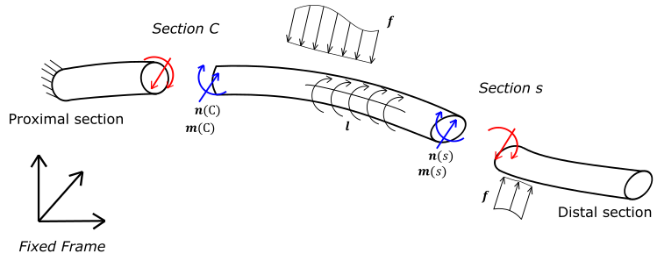
\includegraphics[width=\textwidth]{images/equilibrium}
				\caption{Sections of the beam considered for the static equilibrium.}
			\end{figure}
			\end{columns}
		\end{frame}

        \subsection{BVP}
        \begin{frame}
        	\frametitle{Boundary Value Problem}
			\begin{columns}
			\column{0.5\textwidth}
			\begin{itemize}%[<+->]
  				\item Constraints at the distal plate
  				\begin{itemize}%[<.->]
   					\item External wrench $ \Psi_{ext} = \begin{bmatrix} F \\ M \end{bmatrix}   					 $
   					\item Rod contribution $ \Psi_{i} = \begin{bmatrix} {n_i}_{(L_i)} \\ {m_i}_{(L_i)} \end{bmatrix}   					 $
  				\end{itemize}
  				\item Constraints at the base 
  				\begin{itemize}%[<.->]
   					\item Actuations $ \Psi_{a_i}$
   					\item Joints and geometry 
  				\end{itemize}
 			\end{itemize}
			\vspace{2cm}
			\column{0.5\textwidth}
			\begin{figure}[h]
				\centering
				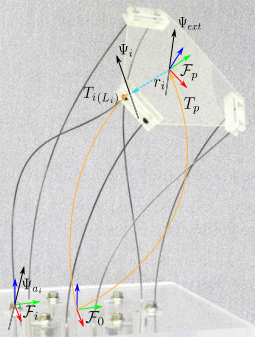
\includegraphics[height=0.7\textheight]{images/BVP}
				\caption{Geometrical and actuation constraints for a Stewart-Gough CPR.}
			\end{figure}
			\end{columns}
		\end{frame}
		
		\subsection{Shooting_method_statics}
        \begin{frame}
        	\frametitle{Shooting Method in statics (Stewart-Gough CPR)}
        	\begin{columns}
			\column{0.5\textwidth}
			\begin{itemize}%[<+->]
  				\item ODE system in statics
  				\item Recursive solution
  				\begin{itemize}			
  					\item Needs an intial guess
  					\item Evaluation on a cost function  
  					\begin{fleqn}
  					\begin{equation}
  						\textbf{\textit{f}} = 
  						\begin{bmatrix}
  							\sum{ {{n}_{i}}_{\left({L}_{i} \right)} }- F \\
  							\sum{ \left[{{p}_{i}}_{\left({L}_{i} \right)} × {{n}_{i}}_{\left({L}_{i} \right)} + {{m}_{i}}_{\left({L}_{i} \right)} \right] } - {p}_{d} × F-M \\
  							{p}_{d} + {R}_{d} {r}_{i} - {{p}_{i}}_{\left({L}_{i} \right)} \\
  							{\left[{{R}_{i}^{T}}_{\left({L}_{i} \right)} {R}_{d} - {{R}_{i}}_{\left({L}_{i} \right)} {R}_{d}^{T} \right]}^{V} 
  						\end{bmatrix}
  					\end{equation}\vfill
  					\end{fleqn}
  				\end{itemize}
  				\item Sensitive to initial conditions
 			\end{itemize}
 			%\vspace{2cm}
			\column{0.5\textwidth}
			\begin{figure}[h]
				\centering
				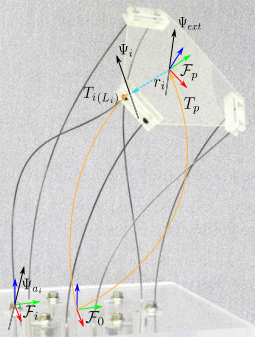
\includegraphics[height=0.7\textheight]{images/BVP}
				\caption{Geometrical and actuation constraints for a Stewart-Gough CPR.}
			\end{figure}
			\end{columns}
		\end{frame}
		
		\subsection{Shooting_method_dynamics}
        \begin{frame}
        	\frametitle{Shooting Method in dynamics}
			\begin{itemize}%[<+->]
				\item PDE system
				\begin{itemize}
					\item Derivative wrt to arc-lenght $ x^{'} = \diffp{x}{s} $
					\item Derivative wrt to time $\dot{x} = \diffp{x}{t} $
				\end{itemize}
				\item From PDE to ODE
				\begin{itemize}
					\item Implicit discretization
					\begin{equation}
						\diffp{x}{t} = {c}_{0} {x}^{(i)} + \sum_{k=1}^{\infty} {\left[{c}_{k} {x}^{\left(i-k \right)} + {d}_{k} {\dot{x}} ^ {\left(i-k \right)} \right]}
					\end{equation}
					\begin{equation}
						\diffp{x}{t} = {c}_{0} {x} ^ {\left(i \right)} + {c}_{1}^{\left(i-1 \right)} {x} ^ {\left(i-1 \right)} + {c}_{2}^{\left(i-2 \right)} {x} ^ {\left(i-2 \right)} + {d}_{1}^{\left(i-1 \right)} \diffp{x^{\left(i-1 \right)}}{t}
					\end{equation}
				\end{itemize}
  				\item Non linear solver
 			\end{itemize}
		\end{frame}
		
		\subsection{Strain_approach_intro}
        \begin{frame}
        	\frametitle{Strain approach, modelling}
			\begin{itemize}%[<+->]
  				\item Modelling of a continuum body in space
  				\begin{itemize}
  					\item With its configuration space $ \textit{C} = SE(3) \times \textit{S} $
  				\end{itemize}
  				\item From assumption on rod deformation
  				\begin{itemize}
  					\item 
  					\item Allowed twist $ \xi_a $
  					\item Prohibited twist $ \xi_c $
  				\end{itemize}
  				\item Discretization of the vector field
 			\end{itemize}
		\end{frame}
		
		\subsection{Strain_approach_deteails}
        \begin{frame}
        	\frametitle{Strain approach, solution}
			\begin{itemize}%[<+->]
  				\item Strain Approach
  				\begin{itemize}
  					\item Details here
  				\end{itemize}
 			\end{itemize}
		\end{frame}
		
		\subsection{ICA_intro}
        \begin{frame}
        	\frametitle{Introduction to the Isogeometric Collocation Method}
			\begin{columns}
			\column{0.5\textwidth}			
			\begin{itemize}%[<+->]
  				\item NURBS curves represent vector field
  				\begin{itemize}
  					\item Control point as degree of freedom
  					\item Basis functions relate influence
  				\end{itemize}
  				\item Cost function
  				\begin{itemize}
  					\item Equilibrium equation evaluated at collocation points
  				\end{itemize}
 			\end{itemize}
 			%\vspace{2cm}
			\column{0.5\textwidth}
			\begin{figure}[h]
				\centering
				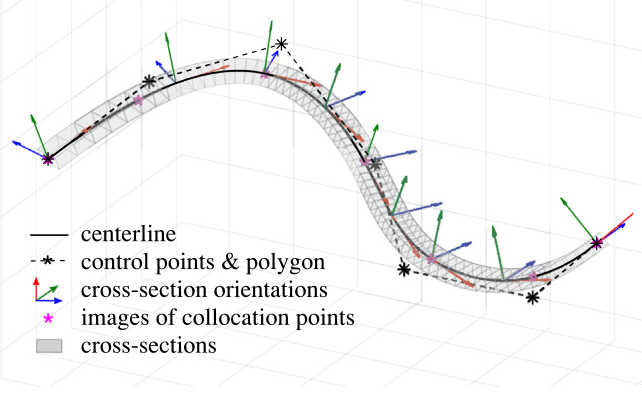
\includegraphics[width=\textwidth]{images/ICA}
				\caption{Rod centerline position and orientation represented with NURBS curves}
			\end{figure}
			\end{columns}
		\end{frame}
		
		\subsection{ICA_details}
        \begin{frame}
        	\frametitle{Properties of the Isogeometric Collocation Method}
			\begin{itemize}%[<+->]
  				\item Less integrations
  				\begin{itemize}
  					\item In statics no integration
  					\item ODE in dynamics
  				\end{itemize}
  				\item Introduces possibility of modelling
  				\begin{itemize}
  					\item Contact between rods
  					\item Changes in shape and or material 
  					\item Rods coupling
  				\end{itemize}
 			\end{itemize}
		\end{frame}

  	\section{Conclusions}
      	\subsection{Conclusions}
        \begin{frame}
        	\begin{itemize}
        		\item 	TODO
        		\begin{itemize}
        			\item TODO
        		\end{itemize}
        	\end{itemize}
        \end{frame}
        	
      	\subsection{Expected_work}
        \begin{frame}
        	\begin{itemize}
        		\item 	TODO
        		\begin{itemize}
        			\item TODO
        		\end{itemize}
        	\end{itemize}
        \end{frame}
        	
        \subsection{References}
        \begin{frame}
        	\begin{itemize}
        		\item 	TODO
        		\begin{itemize}
        			\item TODO
        		\end{itemize}
        	\end{itemize}
        \end{frame}
        	
        \subsection{Thanks}
        \begin{frame}
        	\begin{itemize}
        		\item 	TODO
        		\begin{itemize}
        			\item TODO
        		\end{itemize}
        	\end{itemize}
        \end{frame}
        	

\end{document}
